\documentclass{article}
\usepackage[utf8]{inputenc}
\usepackage{graphicx}
\usepackage{geometry}
\geometry{a4paper, total={16cm, 24cm}, top=2cm}
\usepackage{amsmath}
\usepackage{blindtext}
\graphicspath{ {img/} }
\usepackage{listings}
\usepackage{color}
\usepackage{hyperref}
\hypersetup{
    colorlinks=true,
    linkcolor=blue,
    filecolor=magenta,      
    urlcolor=cyan,
    }
\definecolor{dkgreen}{rgb}{0,0.6,0}
\definecolor{gray}{rgb}{0.5,0.5,0.5}
\definecolor{mauve}{rgb}{0.58,0,0.82}

\lstset{ %frame=tb,
  language=C,
  aboveskip=3mm,
  belowskip=3mm,
  showstringspaces=false,
  columns=flexible,
  numbers=left,
  basicstyle={\small\ttfamily},
  numberstyle=\tiny\color{gray},
  keywordstyle=\color{blue},
  commentstyle=\color{dkgreen},
  stringstyle=\color{mauve},
  breaklines=true,
  breakatwhitespace=true,
  tabsize=3  
}


\title{Week 5 Programming Assignment}
\author{Steffen Petersen | au722120}
\date{October 3rd 2022}

\begin{document}
%\tableofcontents


\maketitle
\section{}
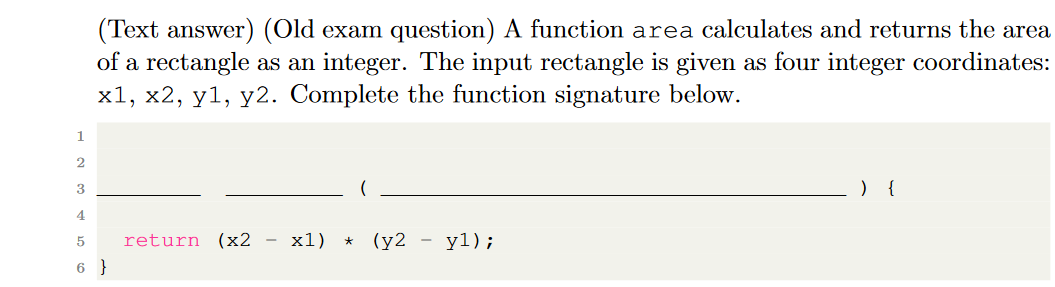
\includegraphics[width=\linewidth, keepaspectratio=true]{task1}
\vspace{2pt}\\
The function should have the following signature:
\begin{lstlisting}
  int area(int x1, int x2, int y1, int y2){
    
    return (x2 - x1) * (y2 - y1);
  }

\end{lstlisting}

\pagebreak
\section{}
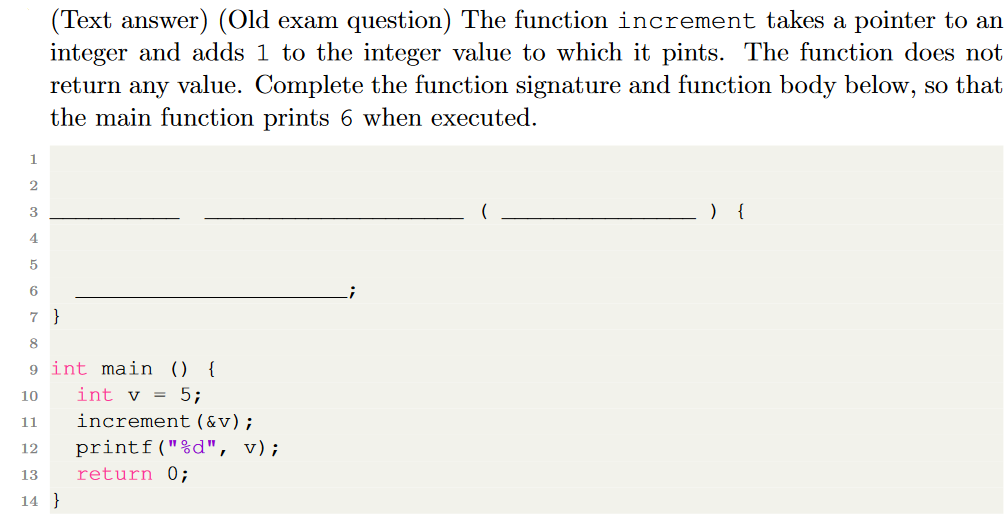
\includegraphics[width=\linewidth, keepaspectratio=true]{task2}
\vspace{2pt}\\
The completed function is below:
\begin{lstlisting}
  void increment(int *in){
    *in += 1;
  }

\end{lstlisting}

\section{}
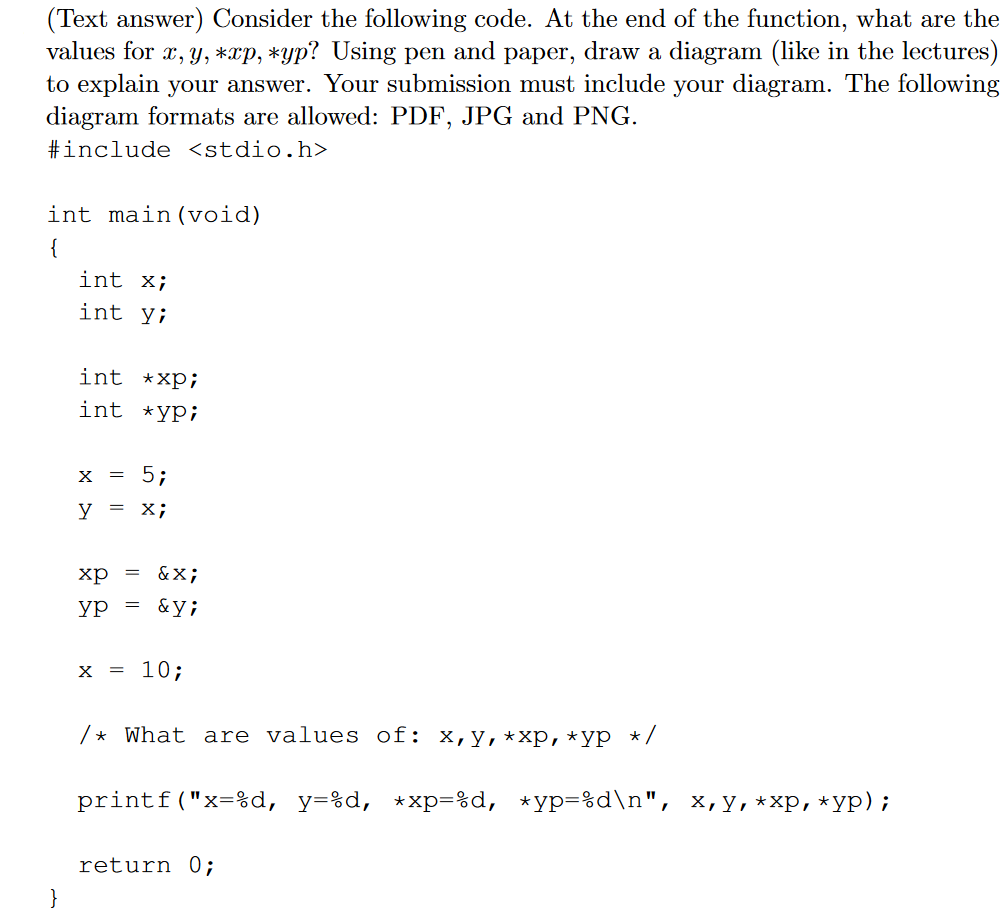
\includegraphics[width=\linewidth, keepaspectratio=true]{task3}
\vspace{2pt}\\
In this code the xp pointer points to x, and the yp pointer points to y.\\
The value of x at the end is 10 and the value of y is 5, and thus the pointers point to 10 and 5 respectively.\\
Below is the diagram over the variables, and this can be found as task3Diagram.png in the /text/img folder.\\
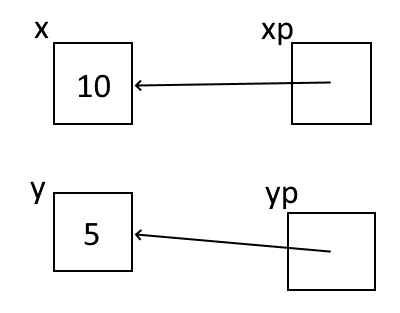
\includegraphics[scale=0.7, keepaspectratio=true]{task3Diagram}


\section{}
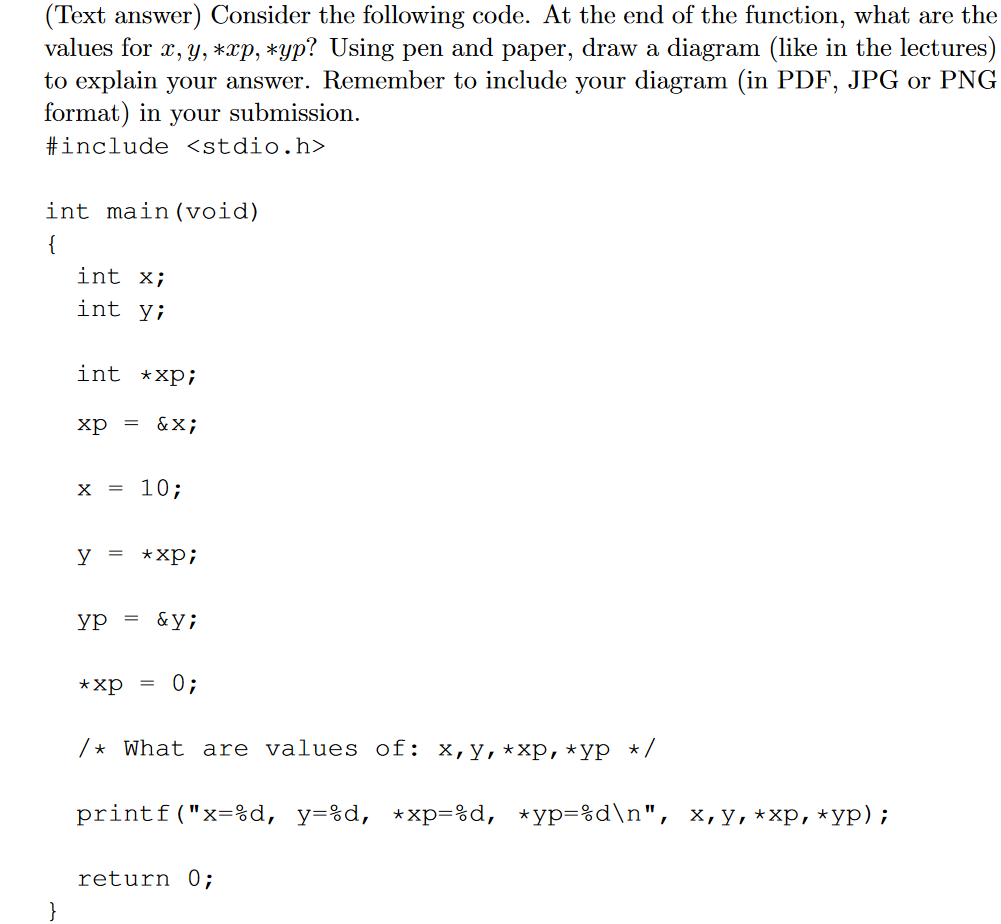
\includegraphics[width=\linewidth, keepaspectratio=true]{task4}
\vspace{2pt}\\
Here the value of x ends at 0, and the value of y ends at 10, xp points to x and yp points to y.\\
Below is the diagram for the code, also included as task4Diagram.png in /text/img\\
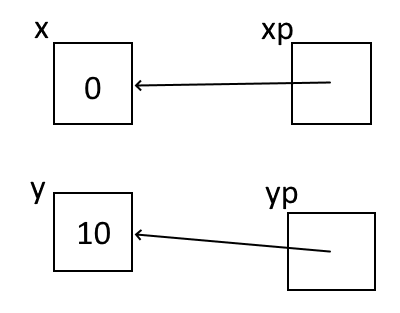
\includegraphics[scale=0.7, keepaspectratio=true]{task4Diagram}

\section{}
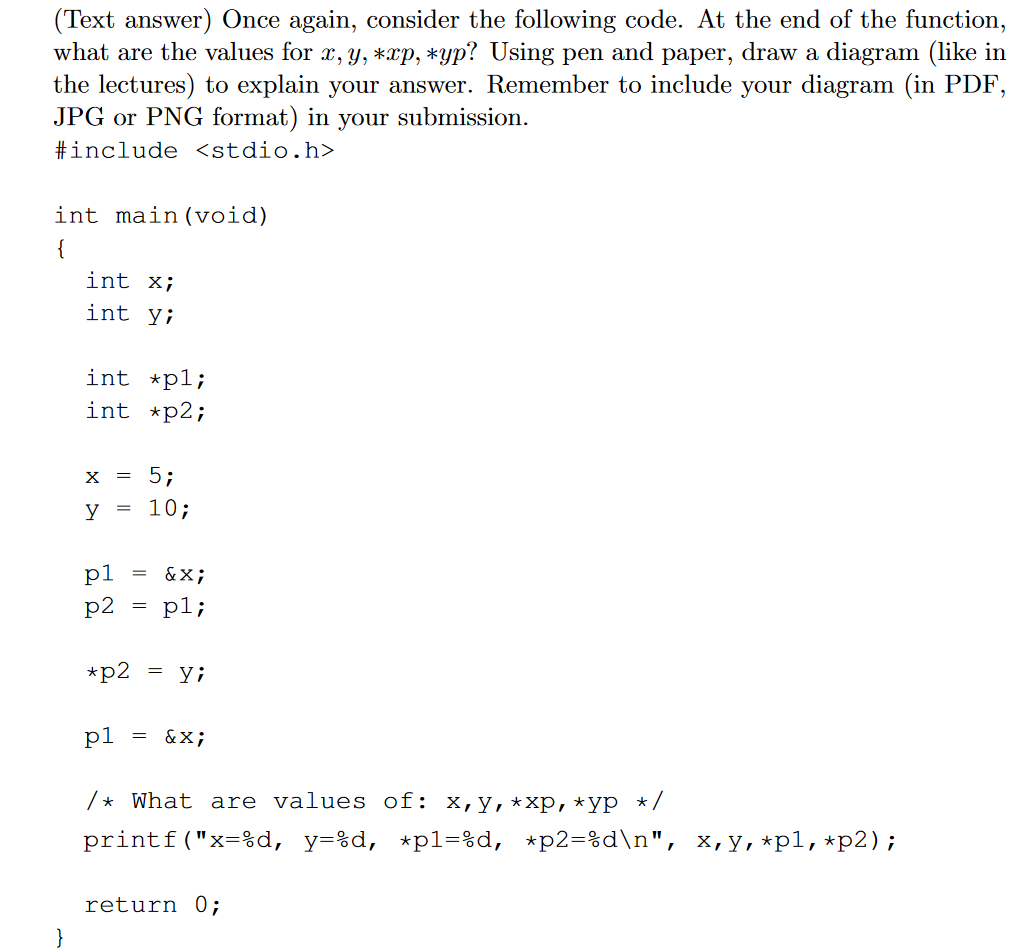
\includegraphics[width=\linewidth, keepaspectratio=true]{task5}
\vspace{2pt}\\
The final value of x would be 10 and the final value of y would be 10, and both pointers point to x.\\
Below is the diagram for the variables, it can be found as task5Diagram.png in /text/img\\
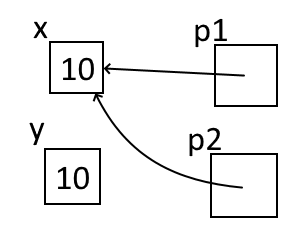
\includegraphics[scale=0.7, keepaspectratio=true]{task5Diagram}


\section{}
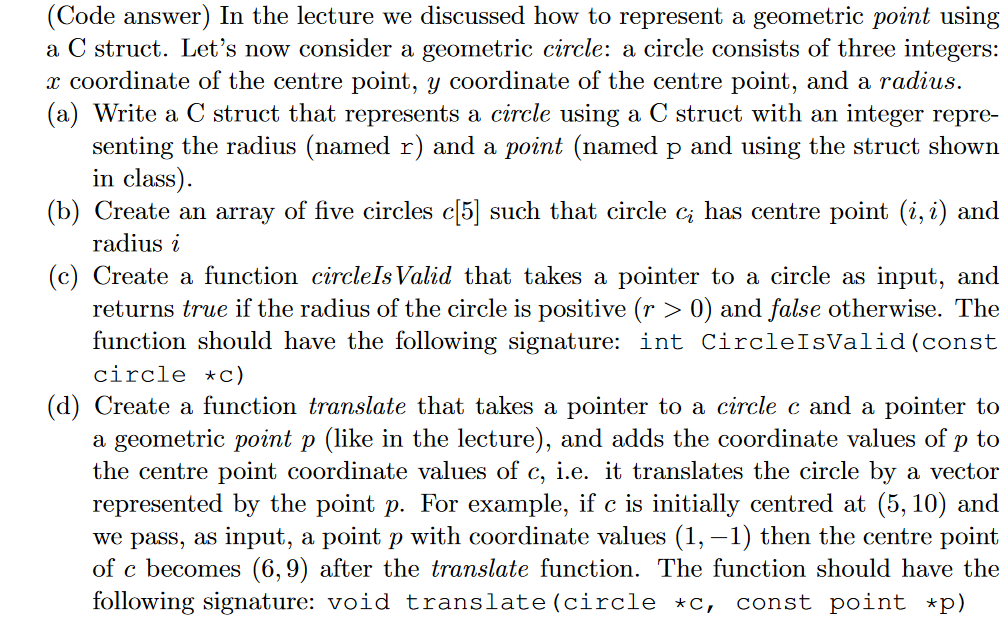
\includegraphics[width=\linewidth, keepaspectratio=true]{task6}
\vspace{2pt}\\
The edits/answers to this task can be found in the files here in the repository, this one related to circle.h and circle.c


\section{}
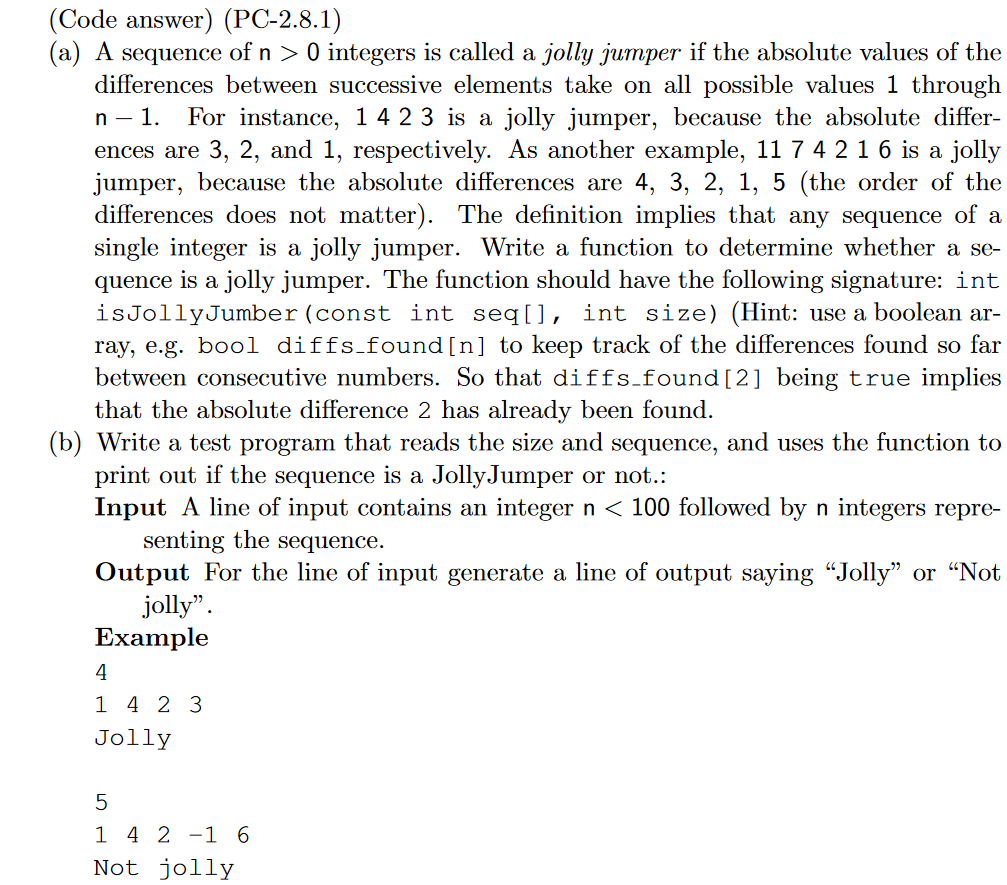
\includegraphics[width=\linewidth, keepaspectratio=true]{task7}
\vspace{2pt}\\


\end{document}